\documentclass[tikz,margin=5mm]{standalone}
\usepackage{amssymb}
\usetikzlibrary{shapes.multipart,positioning,arrows,calc}
\tikzset{
    listnode/.style={
        rectangle split,rectangle split parts=3,draw,rectangle split horizontal,fill=yellow!15
    },
    startnode/.style={
        draw,minimum width=1cm,minimum height=.75cm
    }
}

\begin{document}
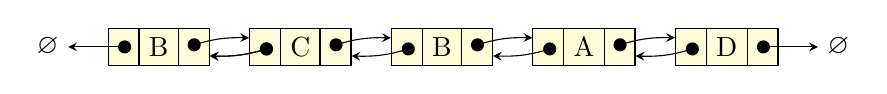
\begin{tikzpicture}[scale=5.0, >=stealth]
\node[] (n1x) {$\varnothing$};
\node[listnode,right=.5cm of n1x] (n1) {\nodepart{second} B};
\node[listnode,right=.5cm of n1] (n2) {\nodepart{second} C};
\node[listnode,right=.5cm of n2] (n3) {\nodepart{second} B};
\node[listnode,right=.5cm of n3] (n4) {\nodepart{second} A};
\node[listnode,right=.5cm of n4] (n5) {\nodepart{second} D};
\node[right=.5cm of n5] (n5x) {$\varnothing$};
\draw[*->] let \p1 = (n1.three), \p2 = (n1.center) in (\x1,\y2) to [bend left=10] (n2);
\draw[*->] let \p1 = (n2.three), \p2 = (n1.center) in (\x1,\y2) to [bend left=10] (n3);
\draw[*->] let \p1 = (n3.three), \p2 = (n1.center) in (\x1,\y2) to [bend left=10] (n4);
\draw[*->] let \p1 = (n4.three), \p2 = (n1.center) in (\x1,\y2) to [bend left=10] (n5);
\draw[*->] let \p1 = (n5.three), \p2 = (n1.center) in (\x1,\y2) to (n5x);

\draw[*->] let \p1 = (n1.one), \p2 = (n1.center) in (\x1+1,\y2) to  (n1x);
\draw[*->] let \p1 = (n2.one), \p2 = (n2.center) in (\x1+1,\y2) to [bend left=10] (n1);
\draw[*->] let \p1 = (n2.one), \p2 = (n2.center) in (\x1+1,\y2) to [bend left=10] (n1);
\draw[*->] let \p1 = (n3.one), \p2 = (n3.center) in (\x1+1,\y2) to [bend left=10] (n2);
\draw[*->] let \p1 = (n4.one), \p2 = (n4.center) in (\x1+1,\y2) to [bend left=10] (n3);
\draw[*->] let \p1 = (n5.one), \p2 = (n5.center) in (\x1+1,\y2) to [bend left=10] (n4);
% \draw[*->] let \p1 = (n2.one), \p2 = (n2.center) in (\x1,\y2) -- (n1);
% \draw[*->] let \p1 = (n2.two), \p2 = (n2.center) in (\x1,\y2) -- (n3);
% \draw[*->] let \p1 = (n3.two), \p2 = (n3.center) in (\x1,\y2) -- (n4);
% \draw[*->] let \p1 = (n4.two), \p2 = (n4.center) in (\x1,\y2) -- (n5);
% \draw[*->] let \p1 = (n5.two), \p2 = (n5.center) in (\x1,\y2) -- (n5x);
% \draw[*->] let \p1 = (n2.three), \p2 = (n2.center) in (\x1,\y2) -- (n1);
\end{tikzpicture}




\end{document}
    


